\documentclass[a4paper, 11pt]{article}
\usepackage{graphicx}
\usepackage{amsmath}
\usepackage[pdftex]{hyperref}

\usepackage[a4paper, portrait, margin=1in]{geometry}
\usepackage{graphicx}
\usepackage{xcolor,colortbl}
\usepackage{listings}
\usepackage{caption}
\usepackage{comment}
\usepackage{cleveref}

\captionsetup[lstlisting]{position=bottom}

\definecolor{Gray}{gray}{0.85}
\definecolor{pblue}{rgb}{0.13,0.13,1}
\definecolor{pgreen}{rgb}{0,0.5,0}
\definecolor{pred}{rgb}{0.9,0,0}
\definecolor{pgrey}{rgb}{0.46,0.45,0.48}

\usepackage{listings}
\lstset{language=Java,
  showspaces=false,
  showtabs=false,
  breaklines=true,
  showstringspaces=false,
  breakatwhitespace=true,
  commentstyle=\color{pgreen},
  keywordstyle=\color{pblue},
  stringstyle=\color{pred},
  basicstyle=\ttfamily,
  moredelim=[il][\textcolor{pgrey}]{$$},
  moredelim=[is][\textcolor{pgrey}]{\%\%}{\%\%}
}


% Lengths and indenting
\setlength{\textwidth}{16.5cm}
\setlength{\marginparwidth}{1.5cm}
\setlength{\parindent}{0cm}
\setlength{\parskip}{0.15cm}
\setlength{\textheight}{22cm}
\setlength{\oddsidemargin}{0cm}
\setlength{\evensidemargin}{\oddsidemargin}
\setlength{\topmargin}{0cm}
\setlength{\headheight}{0cm}
\setlength{\headsep}{0cm}

\renewcommand{\familydefault}{\sfdefault}

\title{Data Mining: Learning from Large Data Sets - Fall Semester 2015}
\author{suyifan@student.ethz.ch\\ zjia@student.ethz.ch\\ weixi@student.ethz.ch\\}
\date{\today}

\begin{document}
\maketitle
The goal of this project was to extract the 100 most representative elements from a large image dataset. In other words, what the problem requires is solving K-means on a large dataset, but even using smart initialization techniques (like K-means++) K-means is not fast enough for large datasets. We tried several approaches for solving this problem.

\section*{Extracting Representative Elements} 
The first approach was \emph{K-Means of K-Means}, or in other words, the mapper was running a k-Means algorithm, and the reducer was doing a K-Means based on the output of the mappers. The result was obviously not that much satisfying so we changed our strategy. \\

We then decided to implement an \emph{online k-Means} method using adaptive coresets based on slides as in \cref{fig:formula}. In the mapper, our algorithm sent the selected points in the space (the coresets) to the reducer.
\begin{figure}[!htb]
  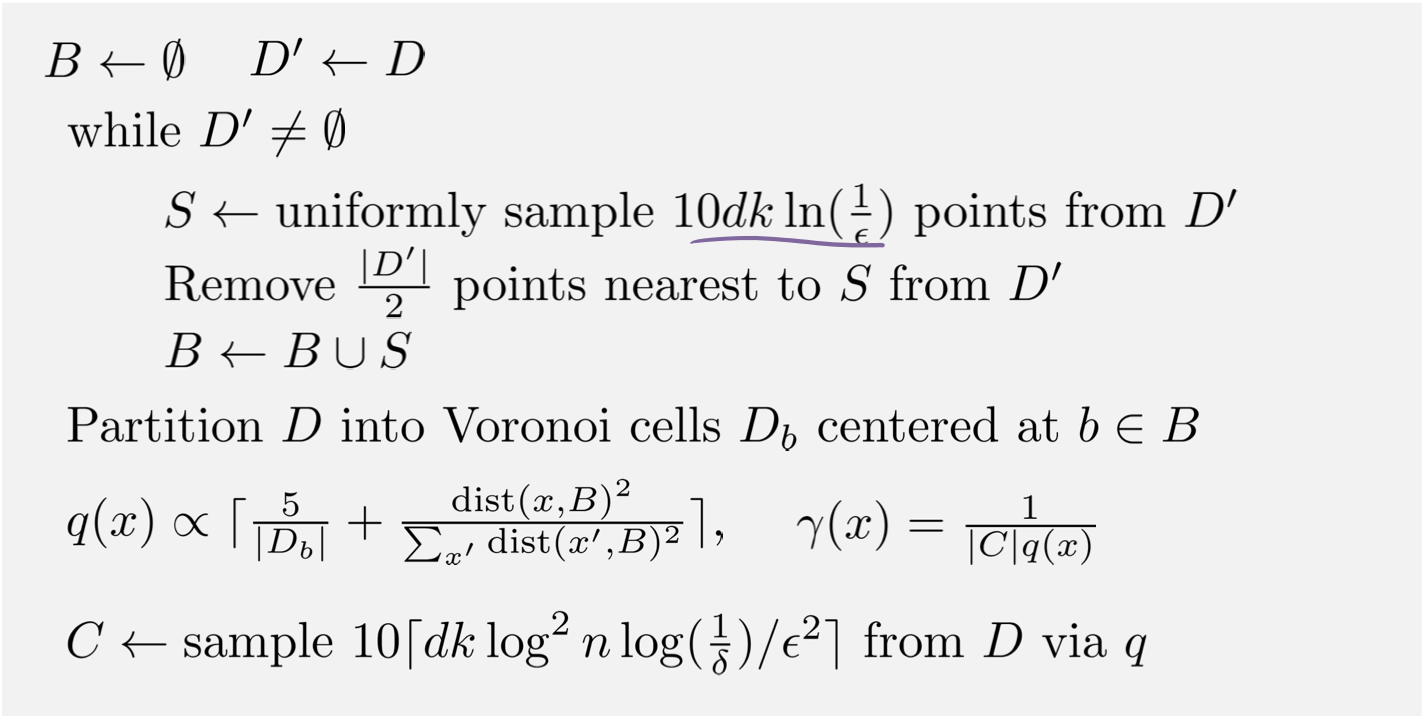
\includegraphics[width=4.5in]{formula}
  \centering
  \caption{Coresets via Adaptive Sampling}
  \label{fig:formula}
\end{figure}
The next thing is to figure out how many points were necessary to sample in order to get a good coreset ($\beta \text{ parameter}$). After finding $\beta$ and with a clever choice of randomly initializing the cluster centers(like K-means++) during reducer phrase we successfully beat the baseline hard with a final score of: \emph{8.85}.

\section*{Team member contribution} 
\begin{itemize}
  \item Yifan SU worked for the parameter selection and report writing;
  \item Xing WEI worked for online k-Means implementation.
  \item Zheng JIA worked for the parameter selection;
\end{itemize}

\end{document} 
